\section{Quadcopter Design}
This section describes the concept designs and build of the quadcopters and parts. 

\subsection{Considerations}
When constructing a quadcopter, special considerations must be made concerning weight, weight distribution and vibrations. There are also many other important design factors, but the mentioned above are the most important for this project.  

\subsection{Components and Manufacture}
In this project a combination of commercially available components and self made parts will be used. Motors, servos, propellers and electronics will be bought.
\\\\
A laser-cutter and 3D-printer is at the teams disposal, which ensures rapid prototyping. At campus, the team has access to a small manual milling machine, lathe and drilling machine. The composite laboratory at campus may also be utilized if needed.

\subsection{Fixed Pitch Quadcopter Design Concepts}
At the beginning of the project, the team had intentions of making two similar quadcopters with less than 11 inch propellers. One fixed pitch quadcopter and one variable pitch quadcopter. The quadcopters should use the same motors, only adding variable pitch mechanisms and servos to achieve maximum similarity and the best foundation for comparison. 
\\\\
An order was placed on motors of the type AEO C20 that could handle both fixed and variable pitch with minor modifications.
When the first orders of motors and mechanisms arrived, they were not usable and the team had spent a good amount of the project budget. Due to limited time and no working fixed pitch quadcopter to test code and control, the team used the resources available and borrowed a set of DJI E600 motors with 12 inch propellers.
\\\\
This was the fastest and most economical way of creating a fixed pitch quadcopter until the team had acquired new variable pitch mechanisms and motors.
\\\\
For the DJI E600 motors, two quadcopter concepts were made. 
\begin{figure}[h]
        \centering
         \begin{minipage}[b]{0.45\textwidth}
            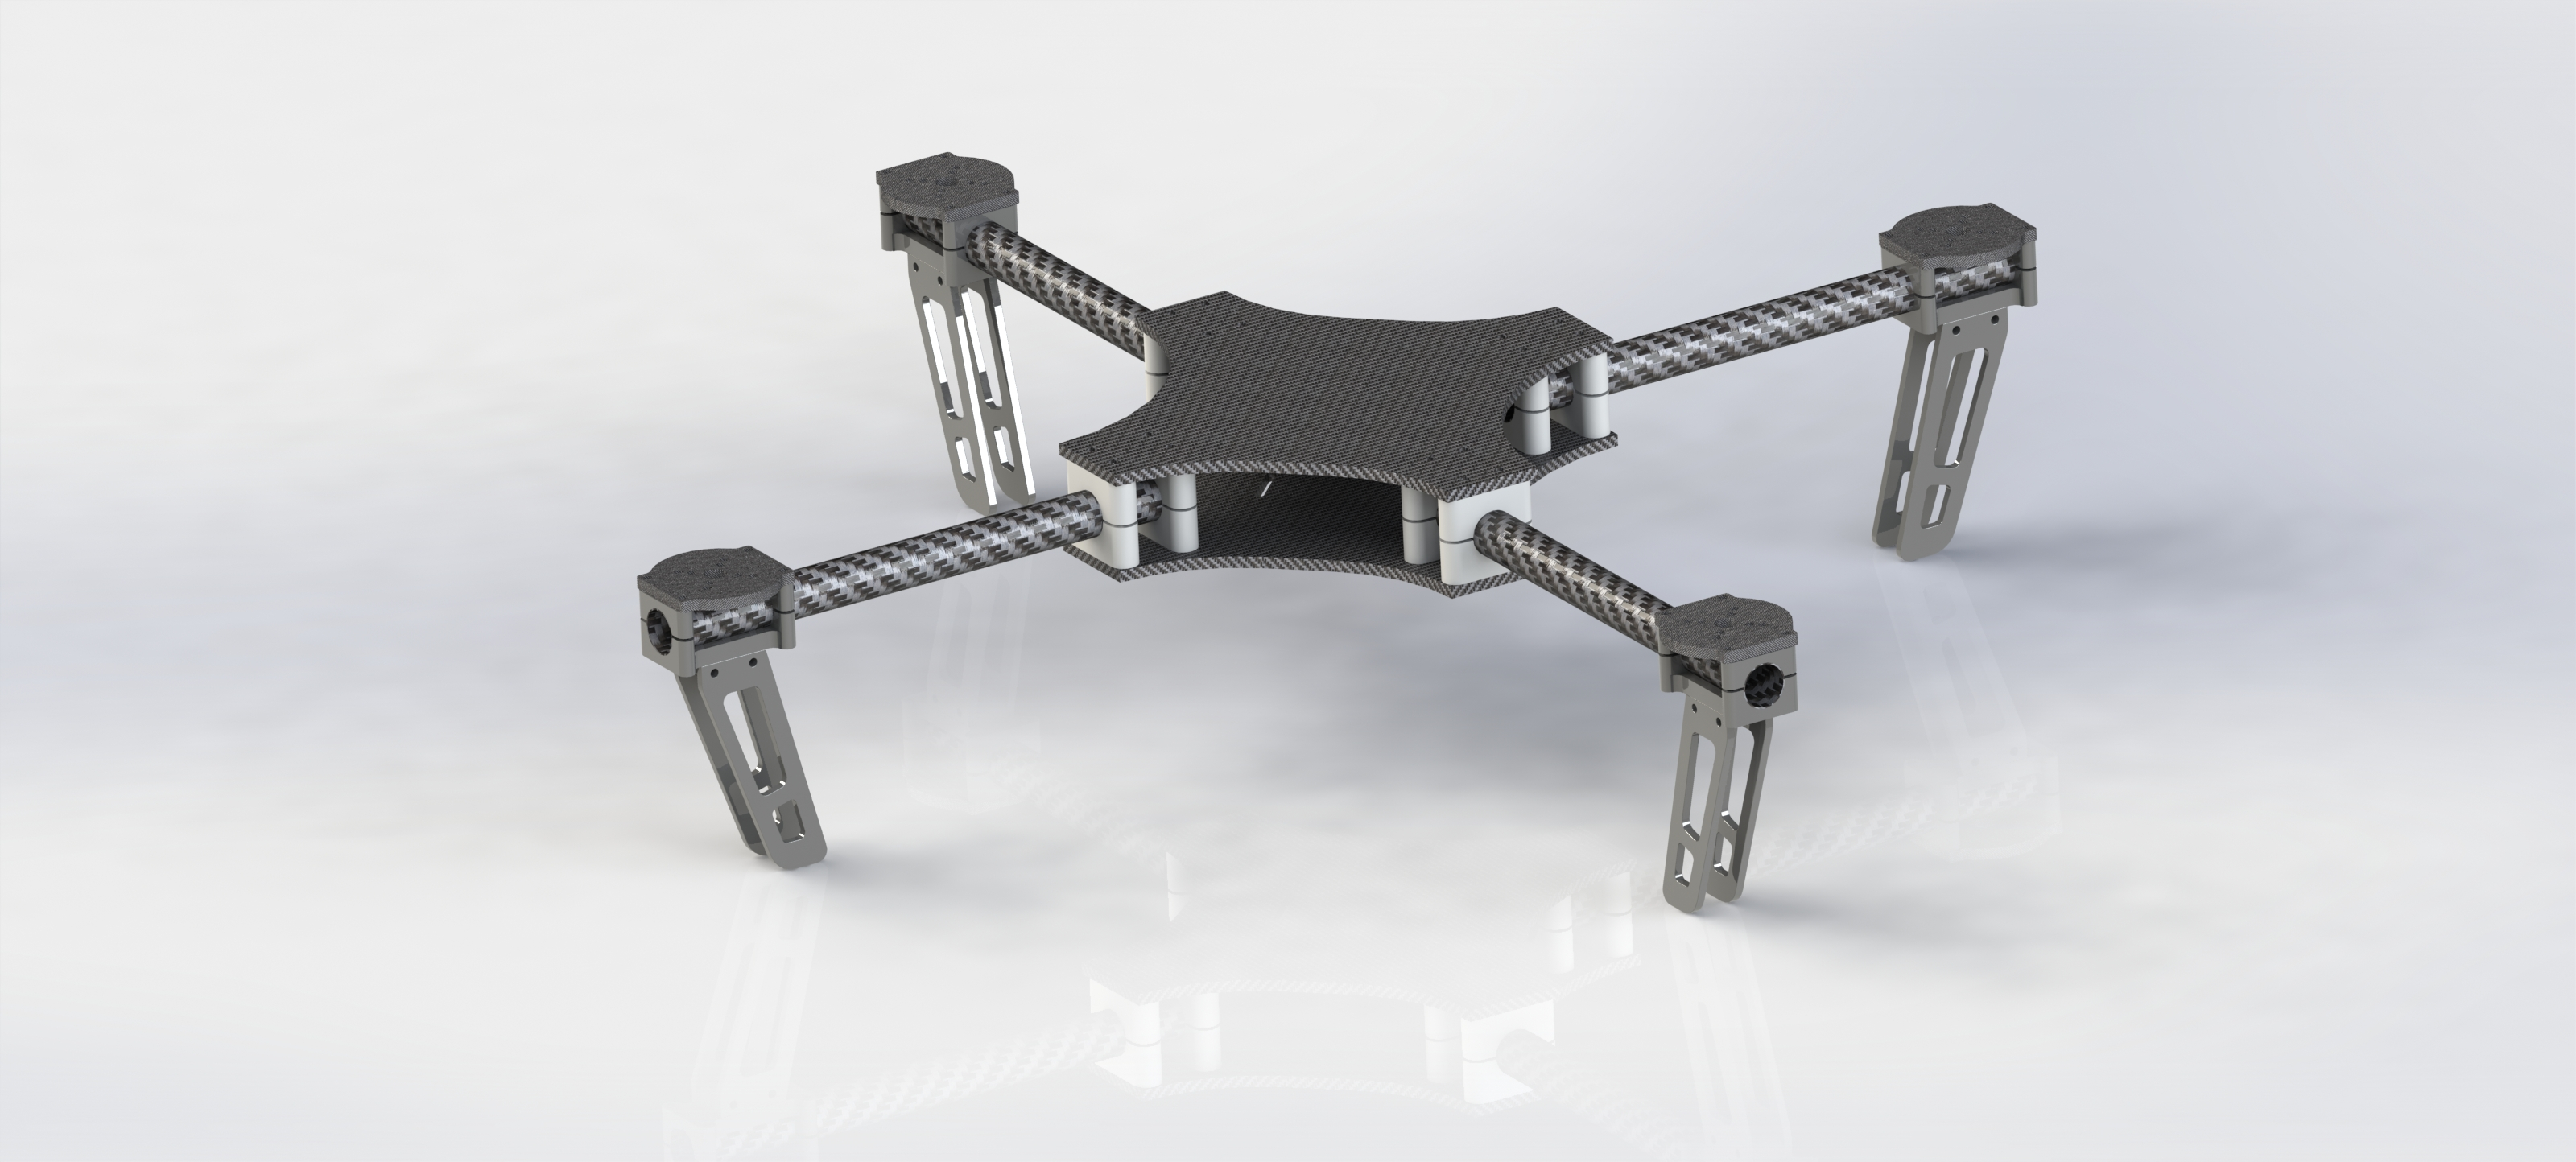
\includegraphics[width = 1\textwidth]{VAPIQ-PICTURES/FixedPitchConceptCarbon}
              \caption{Fixed Pitch Carbon and 3D-print Model}
            \label{fig:CarbonFPQ}
        \end{minipage}
        \hfill
        \begin{minipage}[b]{0.45\textwidth}
            \includegraphics[width = \textwidth]{VAPIQ-PICTURES/FixedPitchso2}
            \caption{Fixed Pitch Plywood Model}
            \label{fig:FPQply}
        \end{minipage}
\end{figure}

\noindent
The design chosen for the fixed pitch quadcopter with 12 inch propellers, was the Plywood Model, see Fig. \ref{fig:FPQply}. This design was the fastest to manufacture and the most economical build. The whole quadcopter frame, support legs and battery holder is made completely with 6,5 mm plywood plates, and can be built in a single session in a laser-cutter. 
\\\\
The build consists of two 6,5 mm main plates glued together with slots for mounting the support legs and top-plate supports. The support legs consists of two parts. One long part, acting as a structural stiffener and as a mount for the battery plate. The second part of the leg is short and perpendicular to the long part for lateral support.
\\\\
For the carbon fixed pitch quadcopter, the frame is made up of two custom cut 2,0 mm carbon fiber plates and 20 mm diameter carbon fiber tube arms. To secure the tube arms, a double set of 3D-printed tube clamps are placed between the custom plates. At the end of the tube arms, there are 3D-printed brackets for the support legs which also acts as a brackets for the motor mount plates. The support legs and motor mount plate, are either 3D-printed or laser-cut, but could also be cut from carbon or glass fiber plates. The battery is placed with a battery strap, through custom slots on the underside of the quadcopter.
\\\\
Since the main objective of this bachelors thesis is not to build a fixed pitch quadcopter, the plywood model was chosen to free time and resources for the variable pitch quadcopter.

\subsection{Fixed Pitch Quadcopter Build}

The plywood quadcopter was made using a Epilog 65W laser-cutter at KIC. After cutting, the quadcopter was glued, assembled and electronics installed (Fig. \ref{fig:Assey}). The E600 motors have a maximum thrust of 1600g/axis, giving the quadcopter a total capacity of 6,4 kg thrust. The assembly has a total weight of 1856g, giving the quadcopter a power to weight ratio of approximately 3,4.

\begin{figure}[h]
        \centering
         \begin{minipage}[b]{0.3\textwidth}
            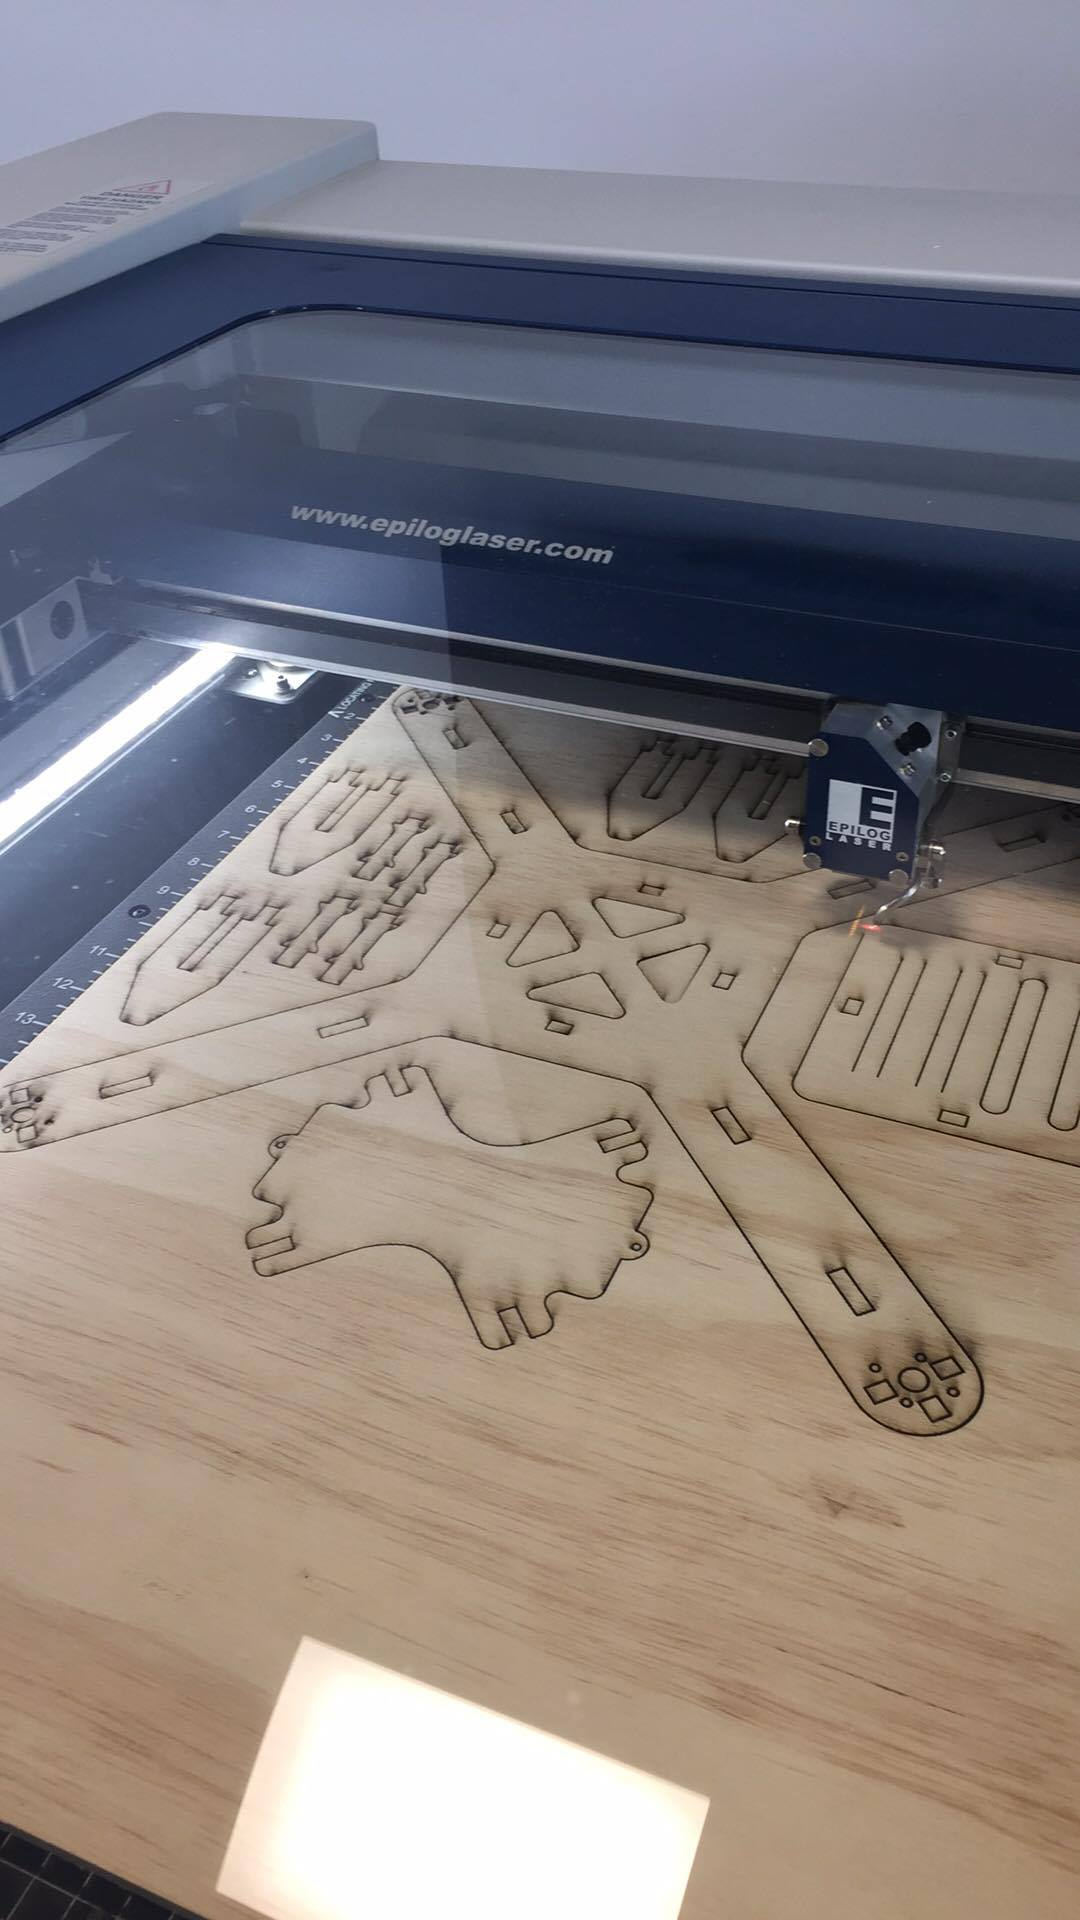
\includegraphics[width = 1\textwidth]{VAPIQ-PICTURES/LaserCut}
              \caption{Cutting quadcopter with Epilog 65W laser}
            \label{fig:CarbonFPQ}
        \end{minipage}
        \hfill
        \begin{minipage}[b]{0.65\textwidth}
            \includegraphics[width = \textwidth]{VAPIQ-PICTURES/AssembledFPQ}
            \caption{Fully assembled fixed pitch quadcopter}
            \label{fig:Assey}
        \end{minipage}
\end{figure}


%%%%%%%%%%
%- Hardware list
%- Mass budget, ish for fixed
%- Power to wheight? ish chack
%%%%%%%%%%
\newpage
\subsection{Variable Pitch Concept 1}

The first concept for the variable pitch quadcopter, was to rebuild a 3DR Arducopter Frame, see Fig. \ref{fig:Arducopter}, and adding helicopter tail pitch mechanisms with mounted motors. The build consists of modifying the tail mechanisms, changing the square arms with carbon fiber tubes, adding tube clamps, leg brackets, servo holders and linkage rods (Fig. \ref{fig:Arducopter}). 
\begin{figure}[h]
        \centering
         \begin{minipage}[b]{0,35\textwidth}
            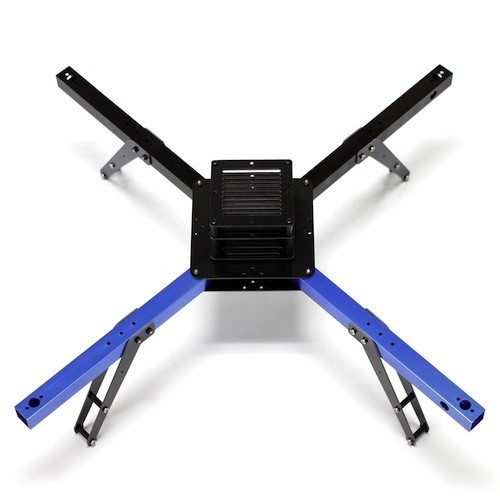
\includegraphics[width =\textwidth, angle =0]{VAPIQ-PICTURES/3DRArducopterCframeKit}
              \caption{3DR Arducopter C Frame Kit}
           \label{fig:Arducopter}
        \end{minipage}
        \hfill
        \begin{minipage}[b]{0.35\textwidth}
            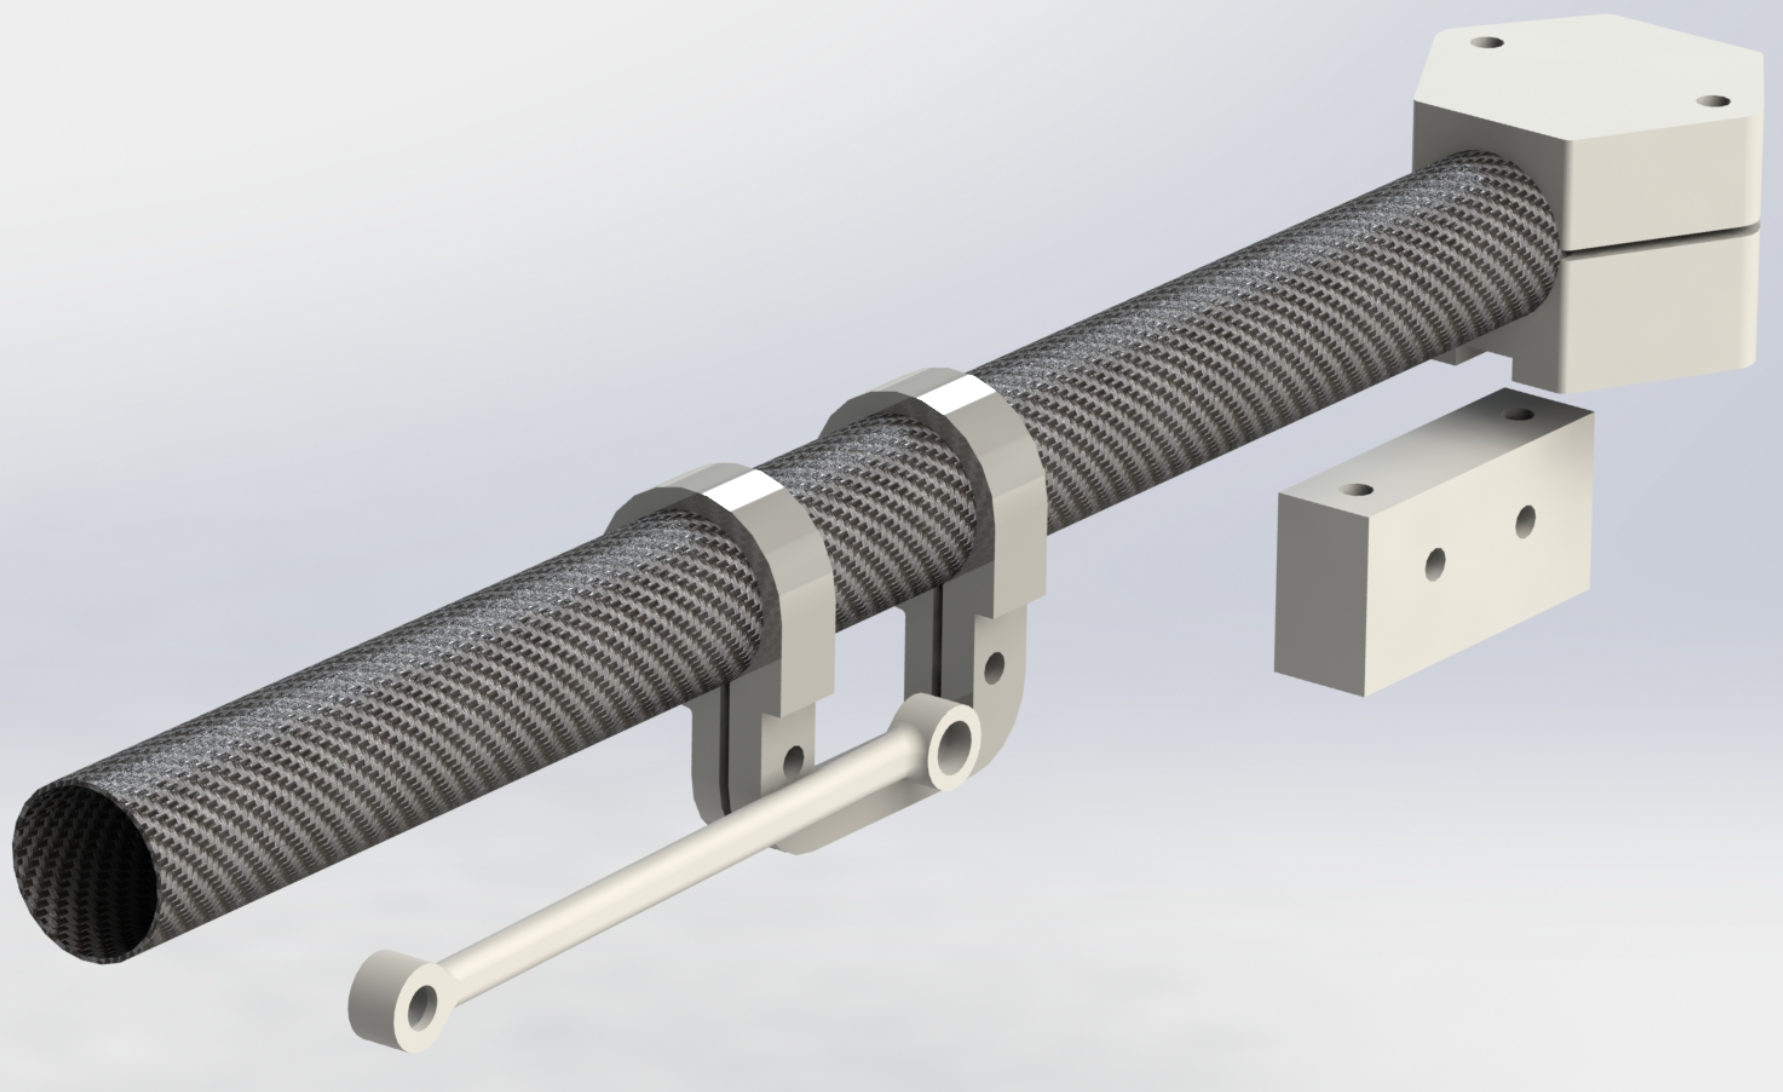
\includegraphics[width = \textwidth]{VAPIQ-PICTURES/ModForVPQ}
            \caption{Parts For Quadcopter Rebuild}
           \label{fig:PartsForArdu}
        \end{minipage}
\end{figure}

\noindent
The tube clamp holds the tube in place and is mounted between the main plates of the frame. Underneath the tube clamp, the leg bracket is mounted. On the tube arms, a servo holder keeps the servo in position, and from the servo, a linkage rod transfers force to adjust the pitch.
\\\\
The legs were moved towards the center of the quadcopter to compensate for the added weight from the motors and mechanisms. The addition of the variable pitch mechanisms and motors severely affects weight distribution, thus increasing inertia and making it harder to maneuver and control. All fasteners used in this build are M3 screws and bolts, and all the parts in (Fig. \ref{fig:PartsForArdu}) excluding the carbon tube are 3D-printed. 
\newpage
\subsection{Helicopter Tail Pitch Mechanism}

Four variable pitch mechanisms were made from RC helicopter tails of the type HK500GT, using steel rods and 880KV motors.

\begin{figure}[h]
        \centering
         \begin{minipage}[b]{0,6\textwidth}
            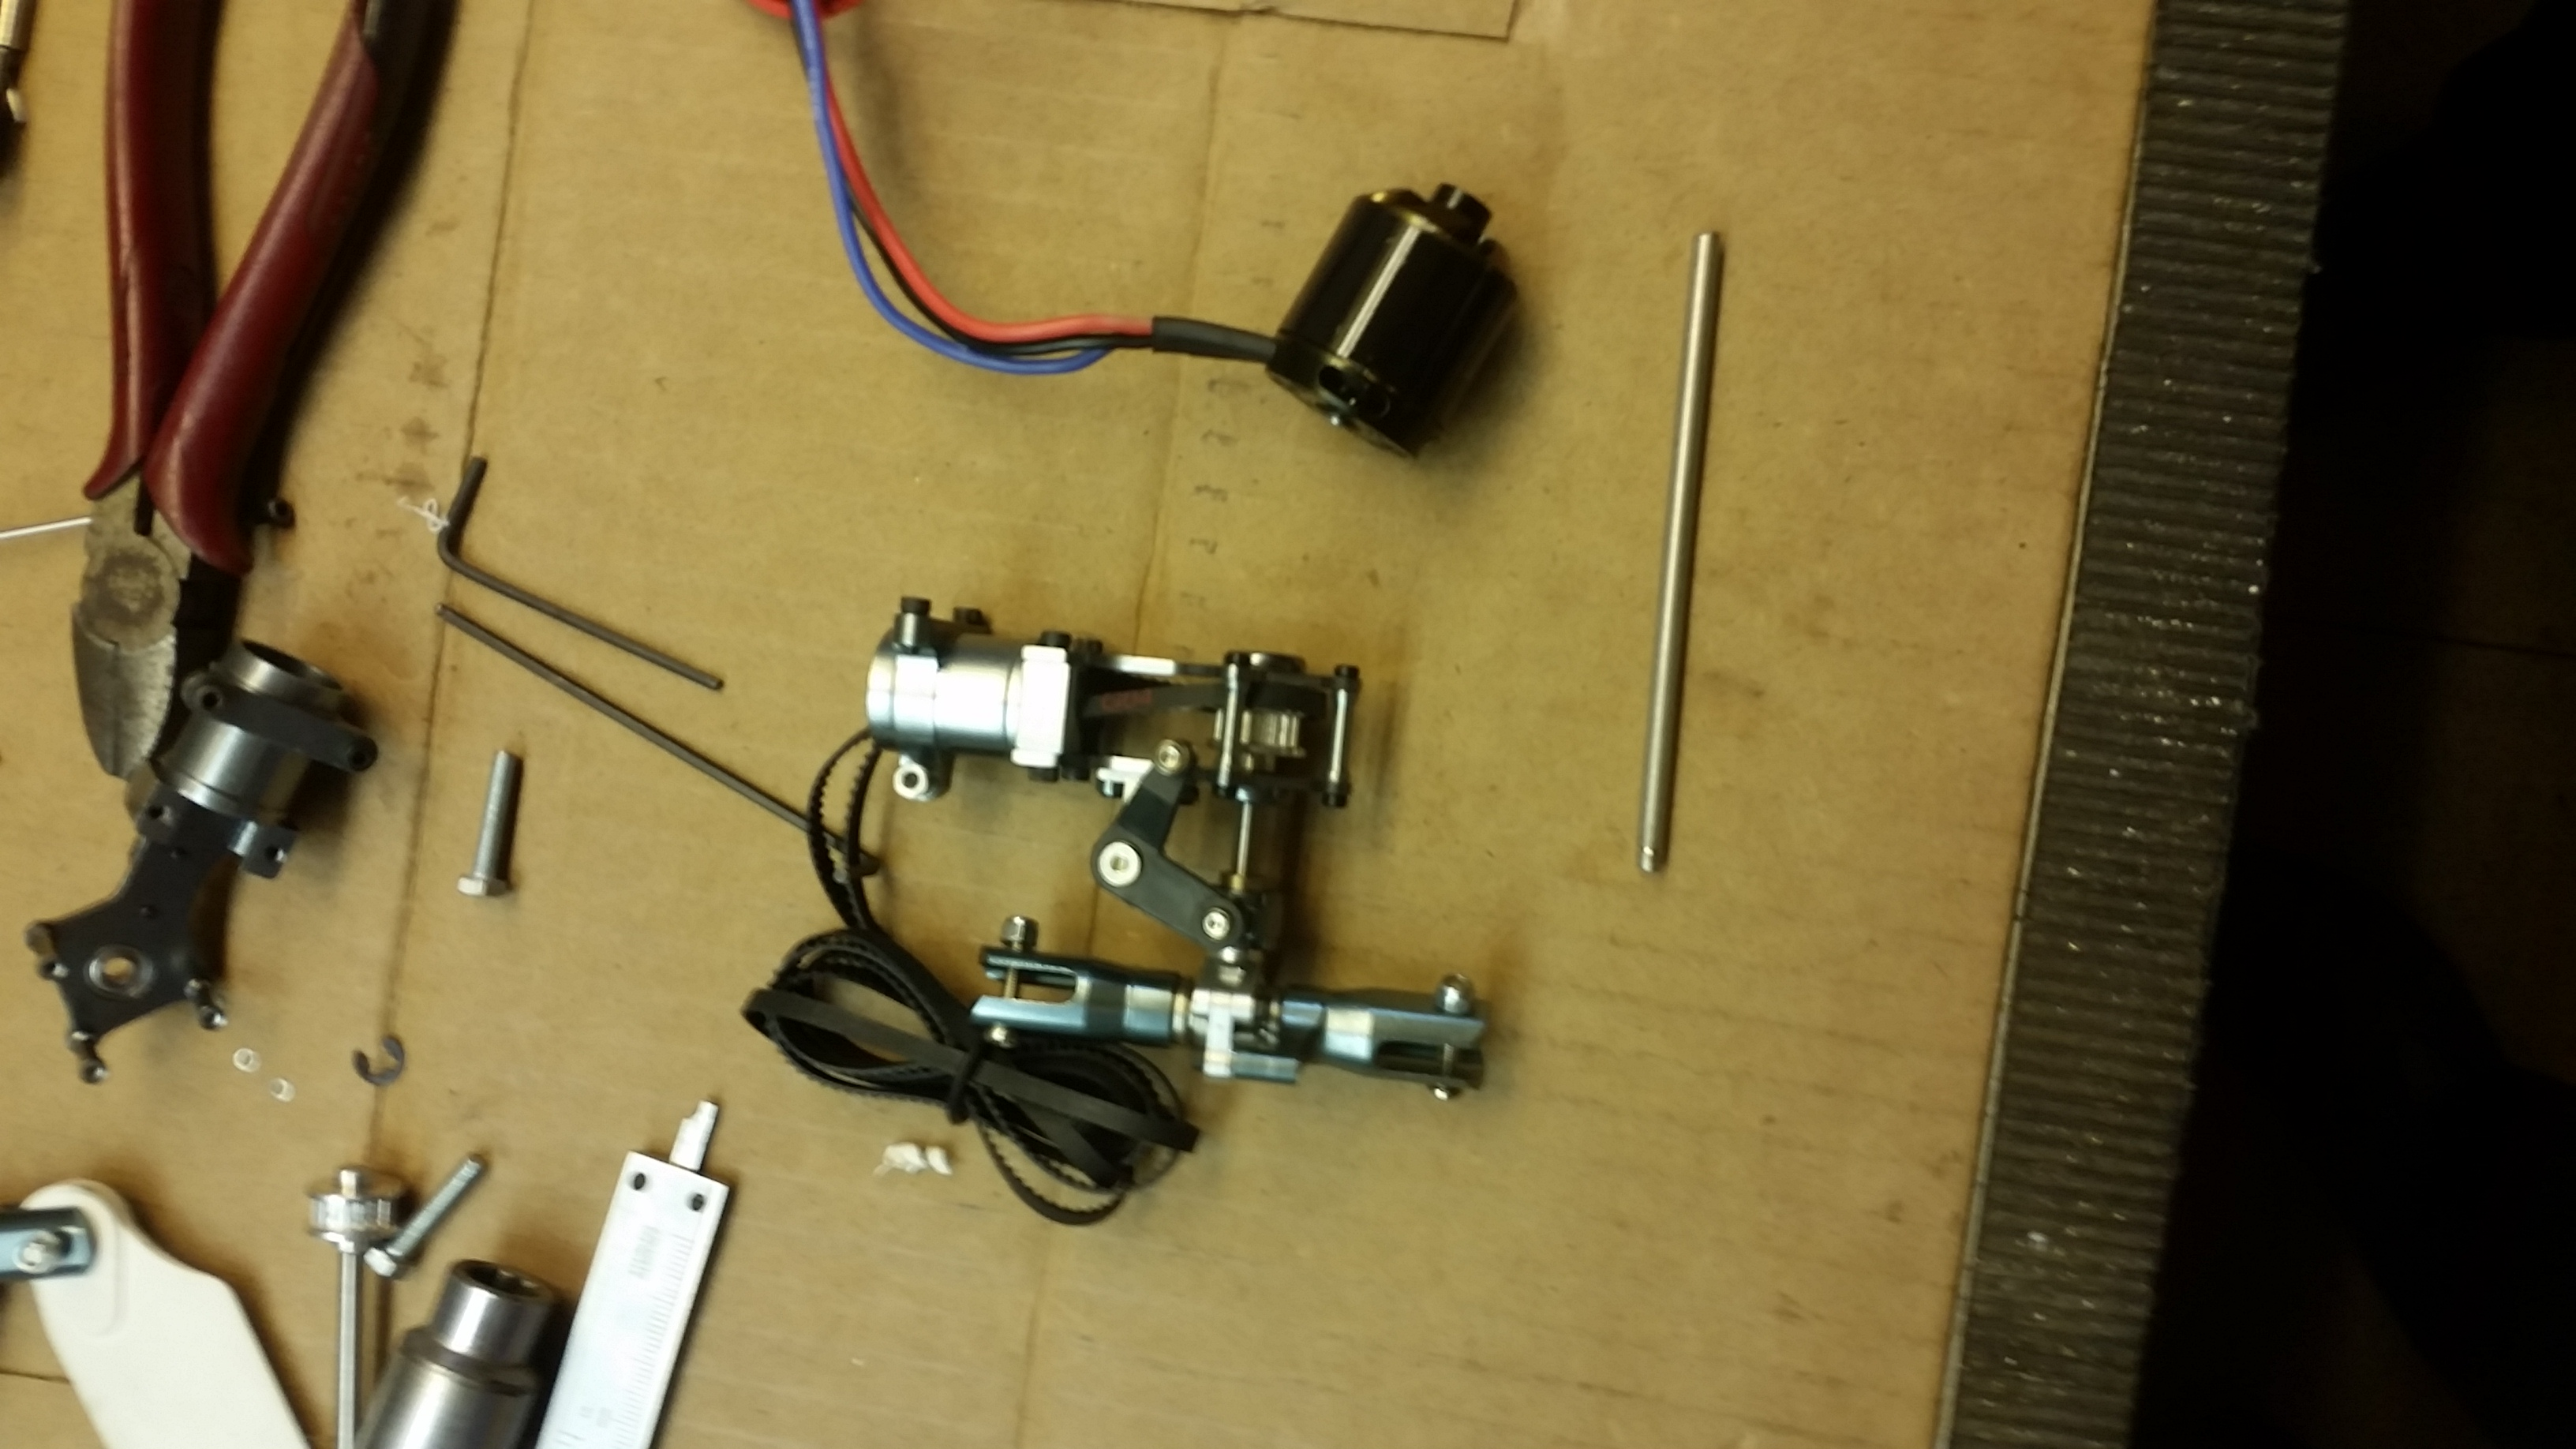
\includegraphics[width =\textwidth, angle =180]{VAPIQ-PICTURES/VPQParts}
              \caption{3DR 880KV motor, 4mm steel rod, hk500gt tail assembly}
            \label{fig:nlknl}
        \end{minipage}
        \hfill
        \begin{minipage}[b]{0.35\textwidth}
            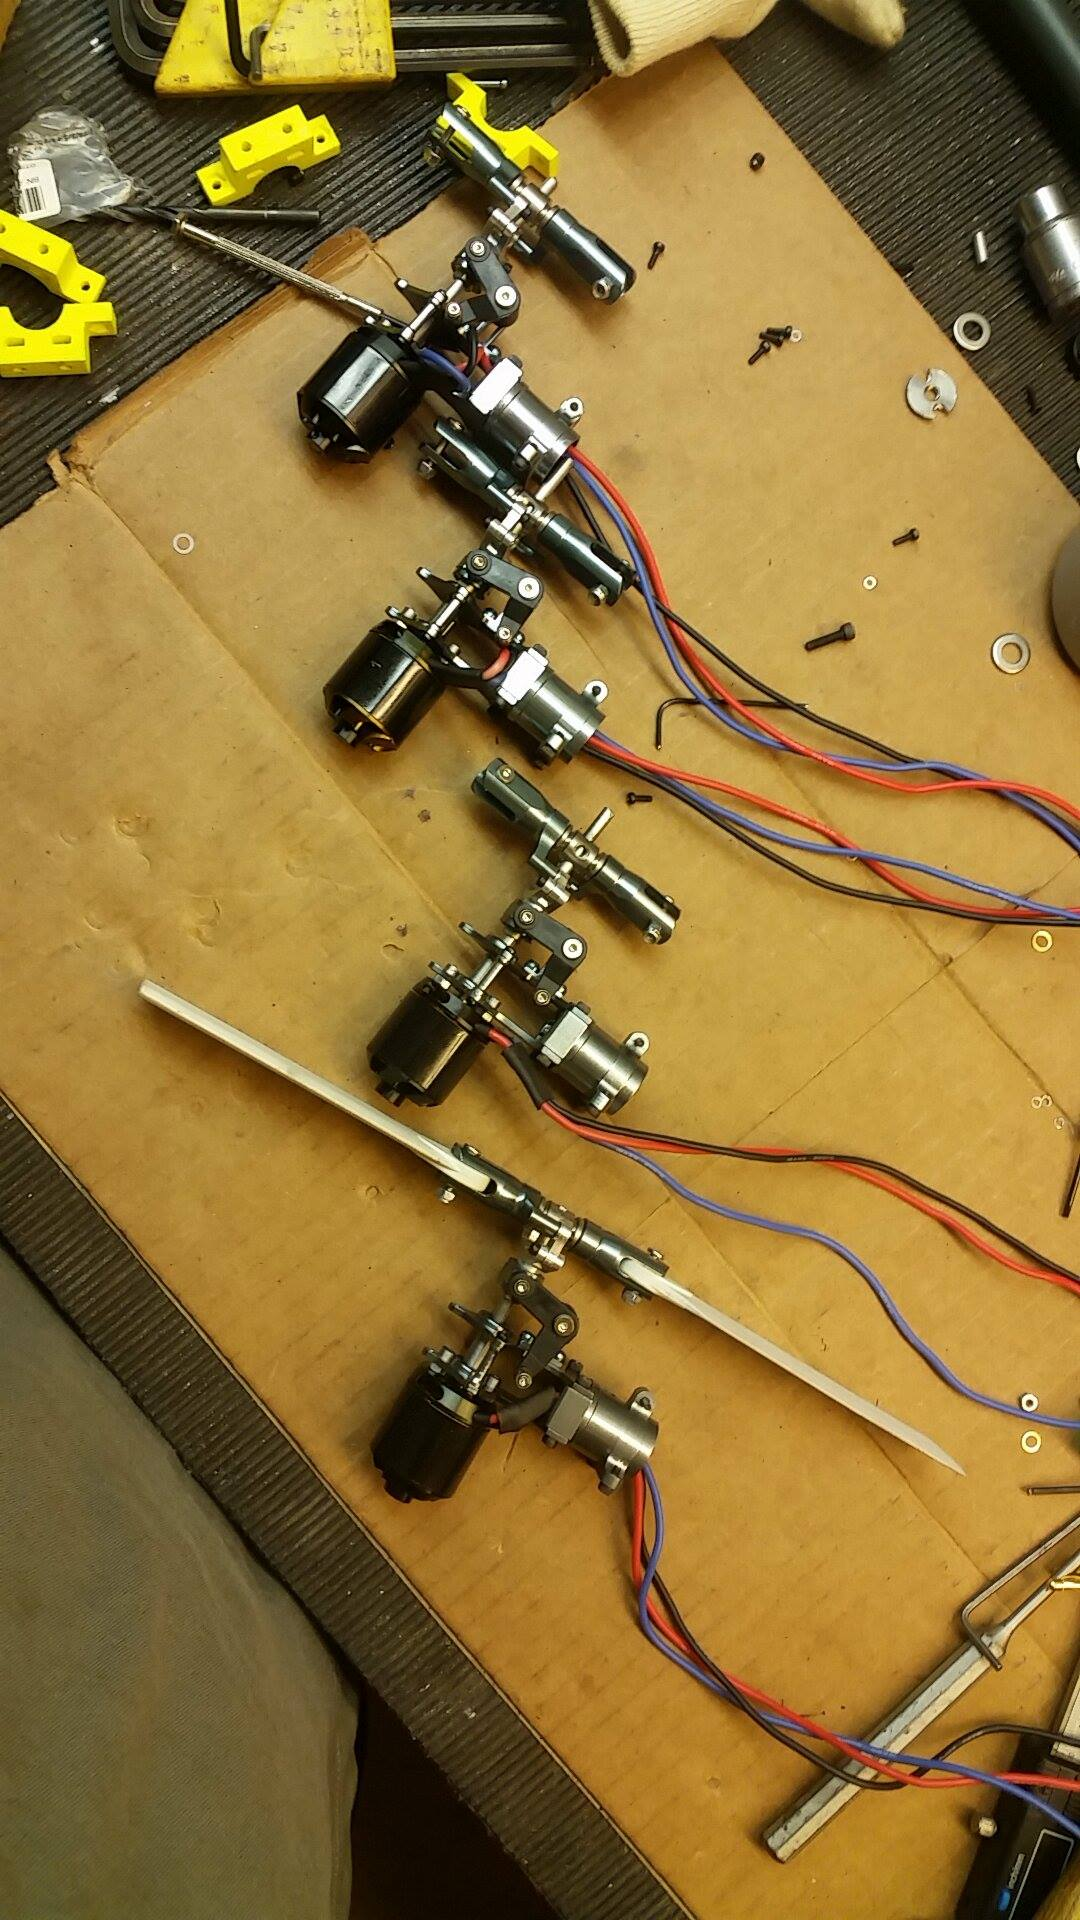
\includegraphics[width = \textwidth]{VAPIQ-PICTURES/VPQassemblies}
            \caption{Assemblies}
            \label{fig:}
        \end{minipage}
\end{figure}

\noindent The mechanisms were built using 4 mm diameter stainless steel rods which runs through the motor and mechanism. The rods are precision cut from a 3 m specimen into 4 pieces of 92,5 mm in length. 

\begin{figure}[H]
        \centering
         \begin{minipage}[b]{0,35\textwidth}
            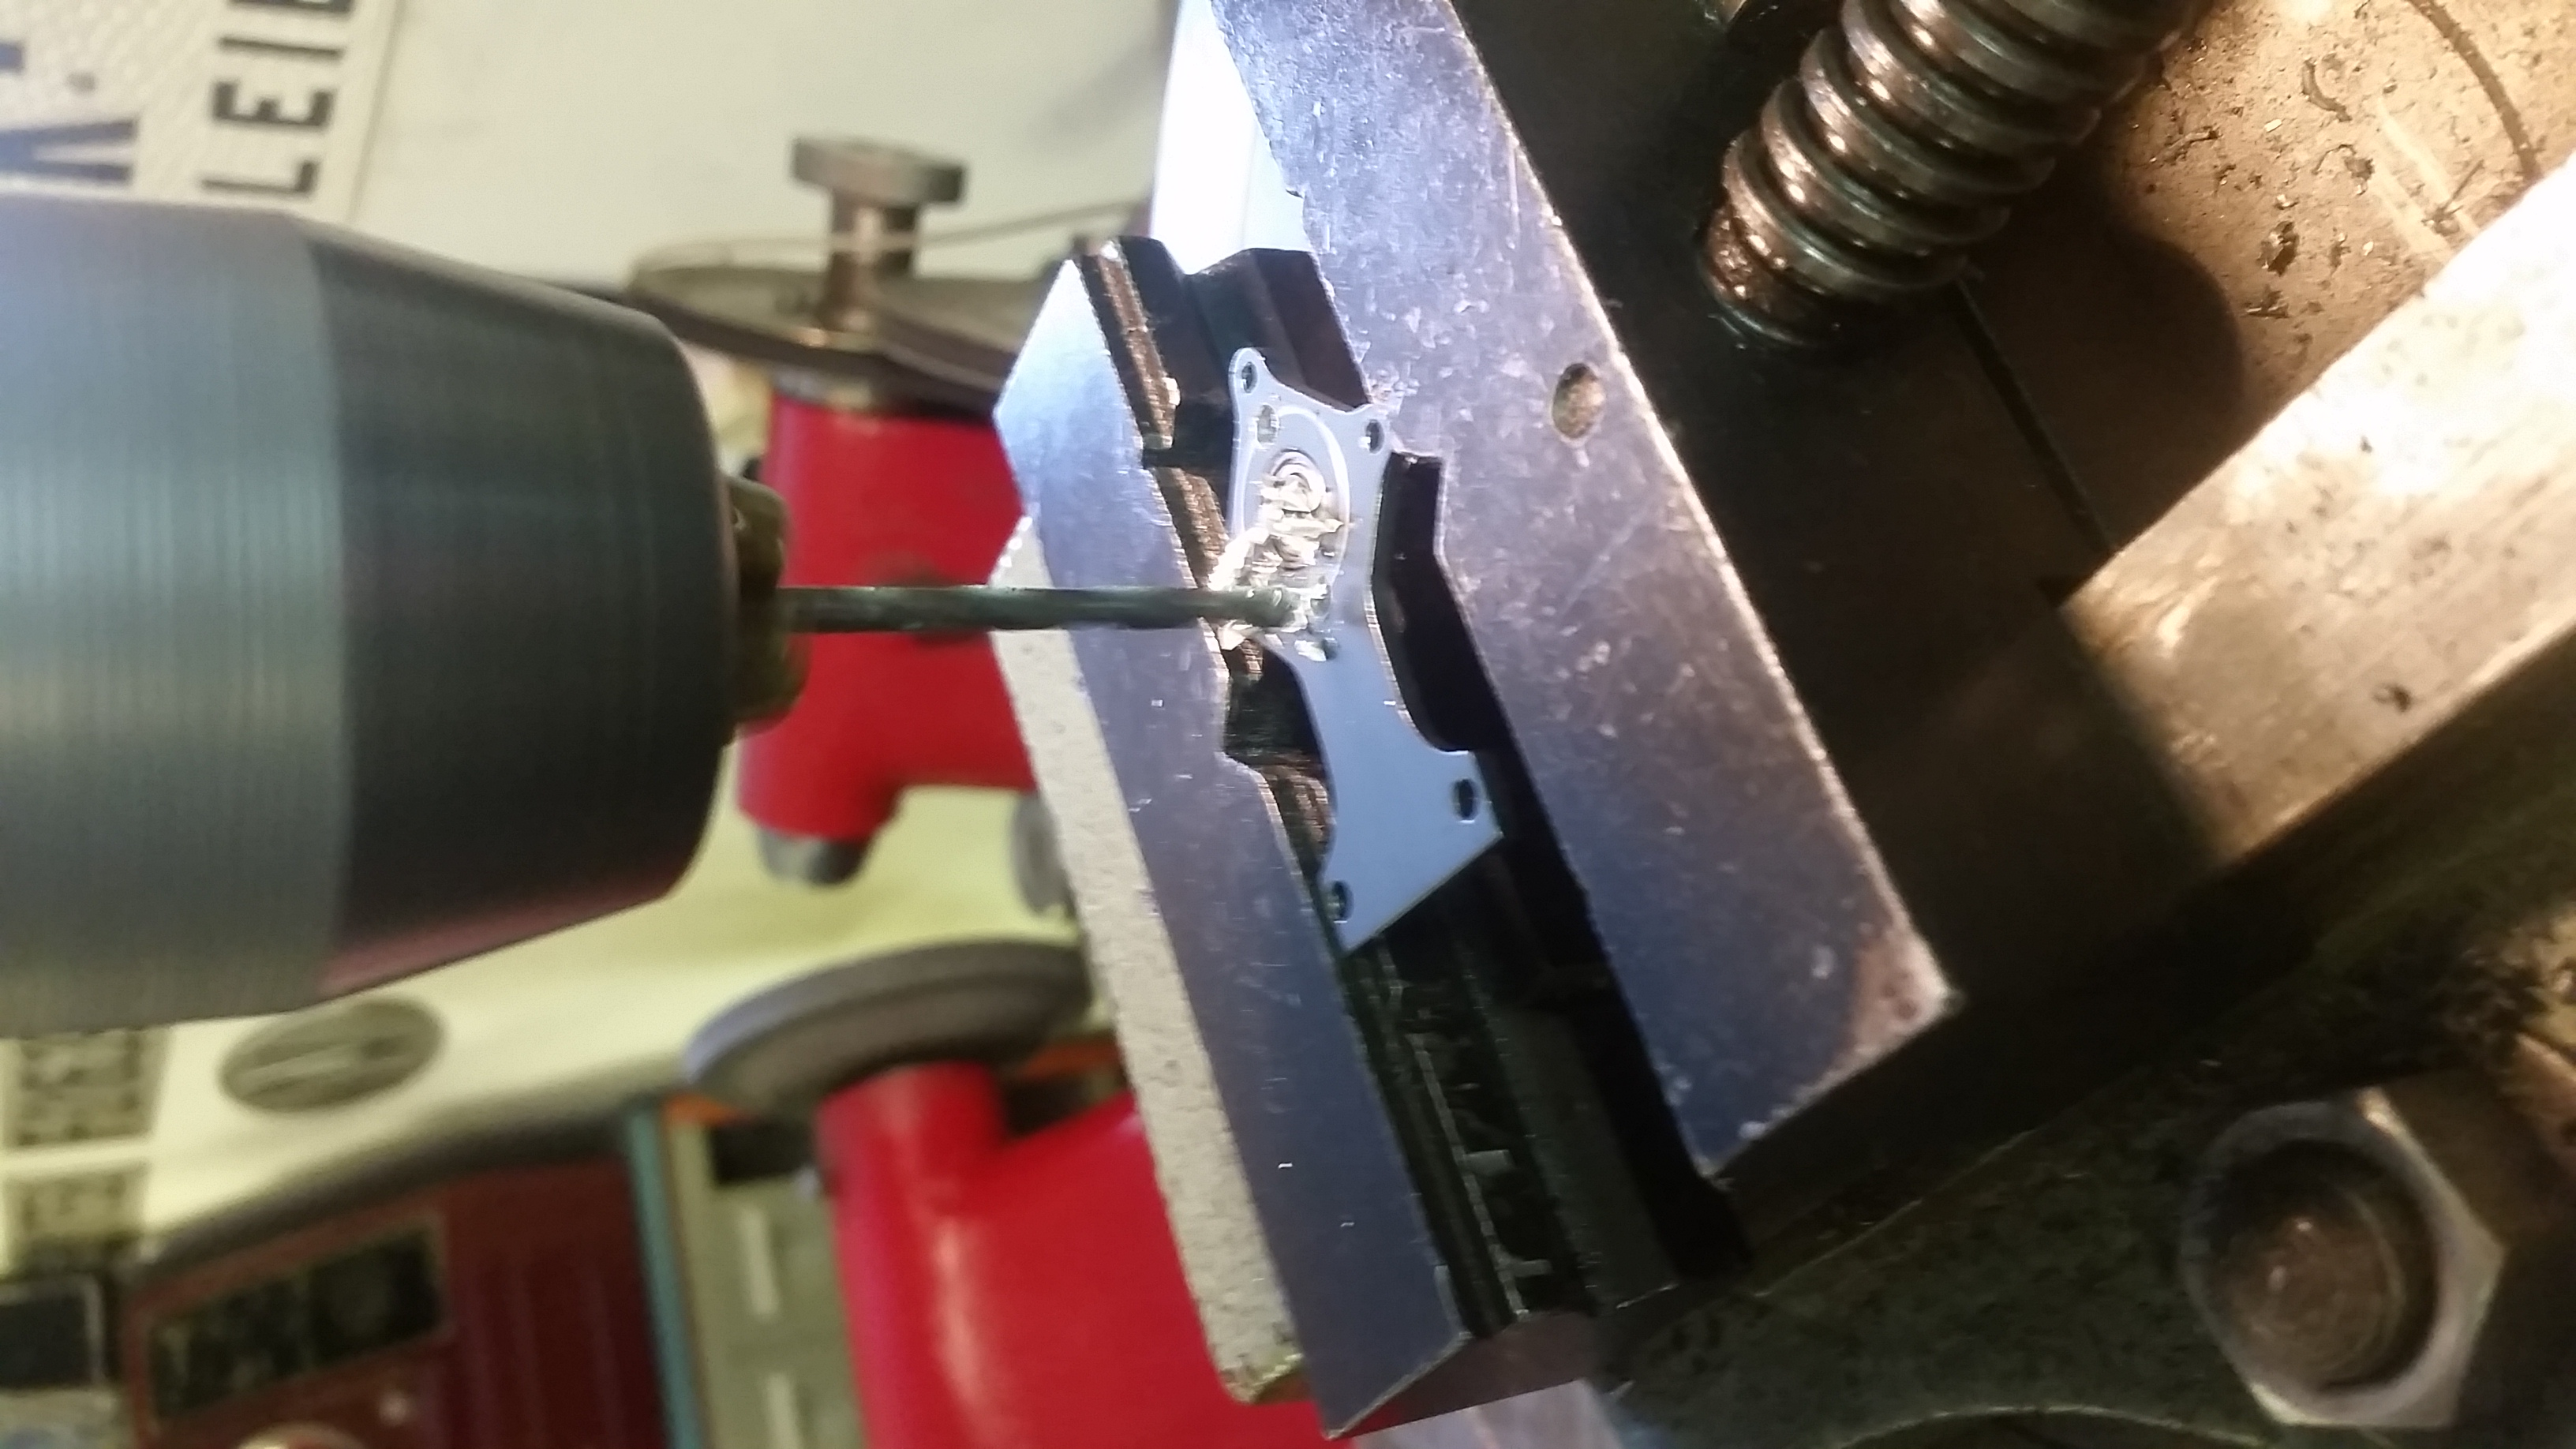
\includegraphics[width =\textwidth, angle =270]{VAPIQ-PICTURES/Drilling}
              \caption{Drilling}
            %\label{fig:nlknl}
        \end{minipage}
        \hfill
        \begin{minipage}[b]{0.35\textwidth}
            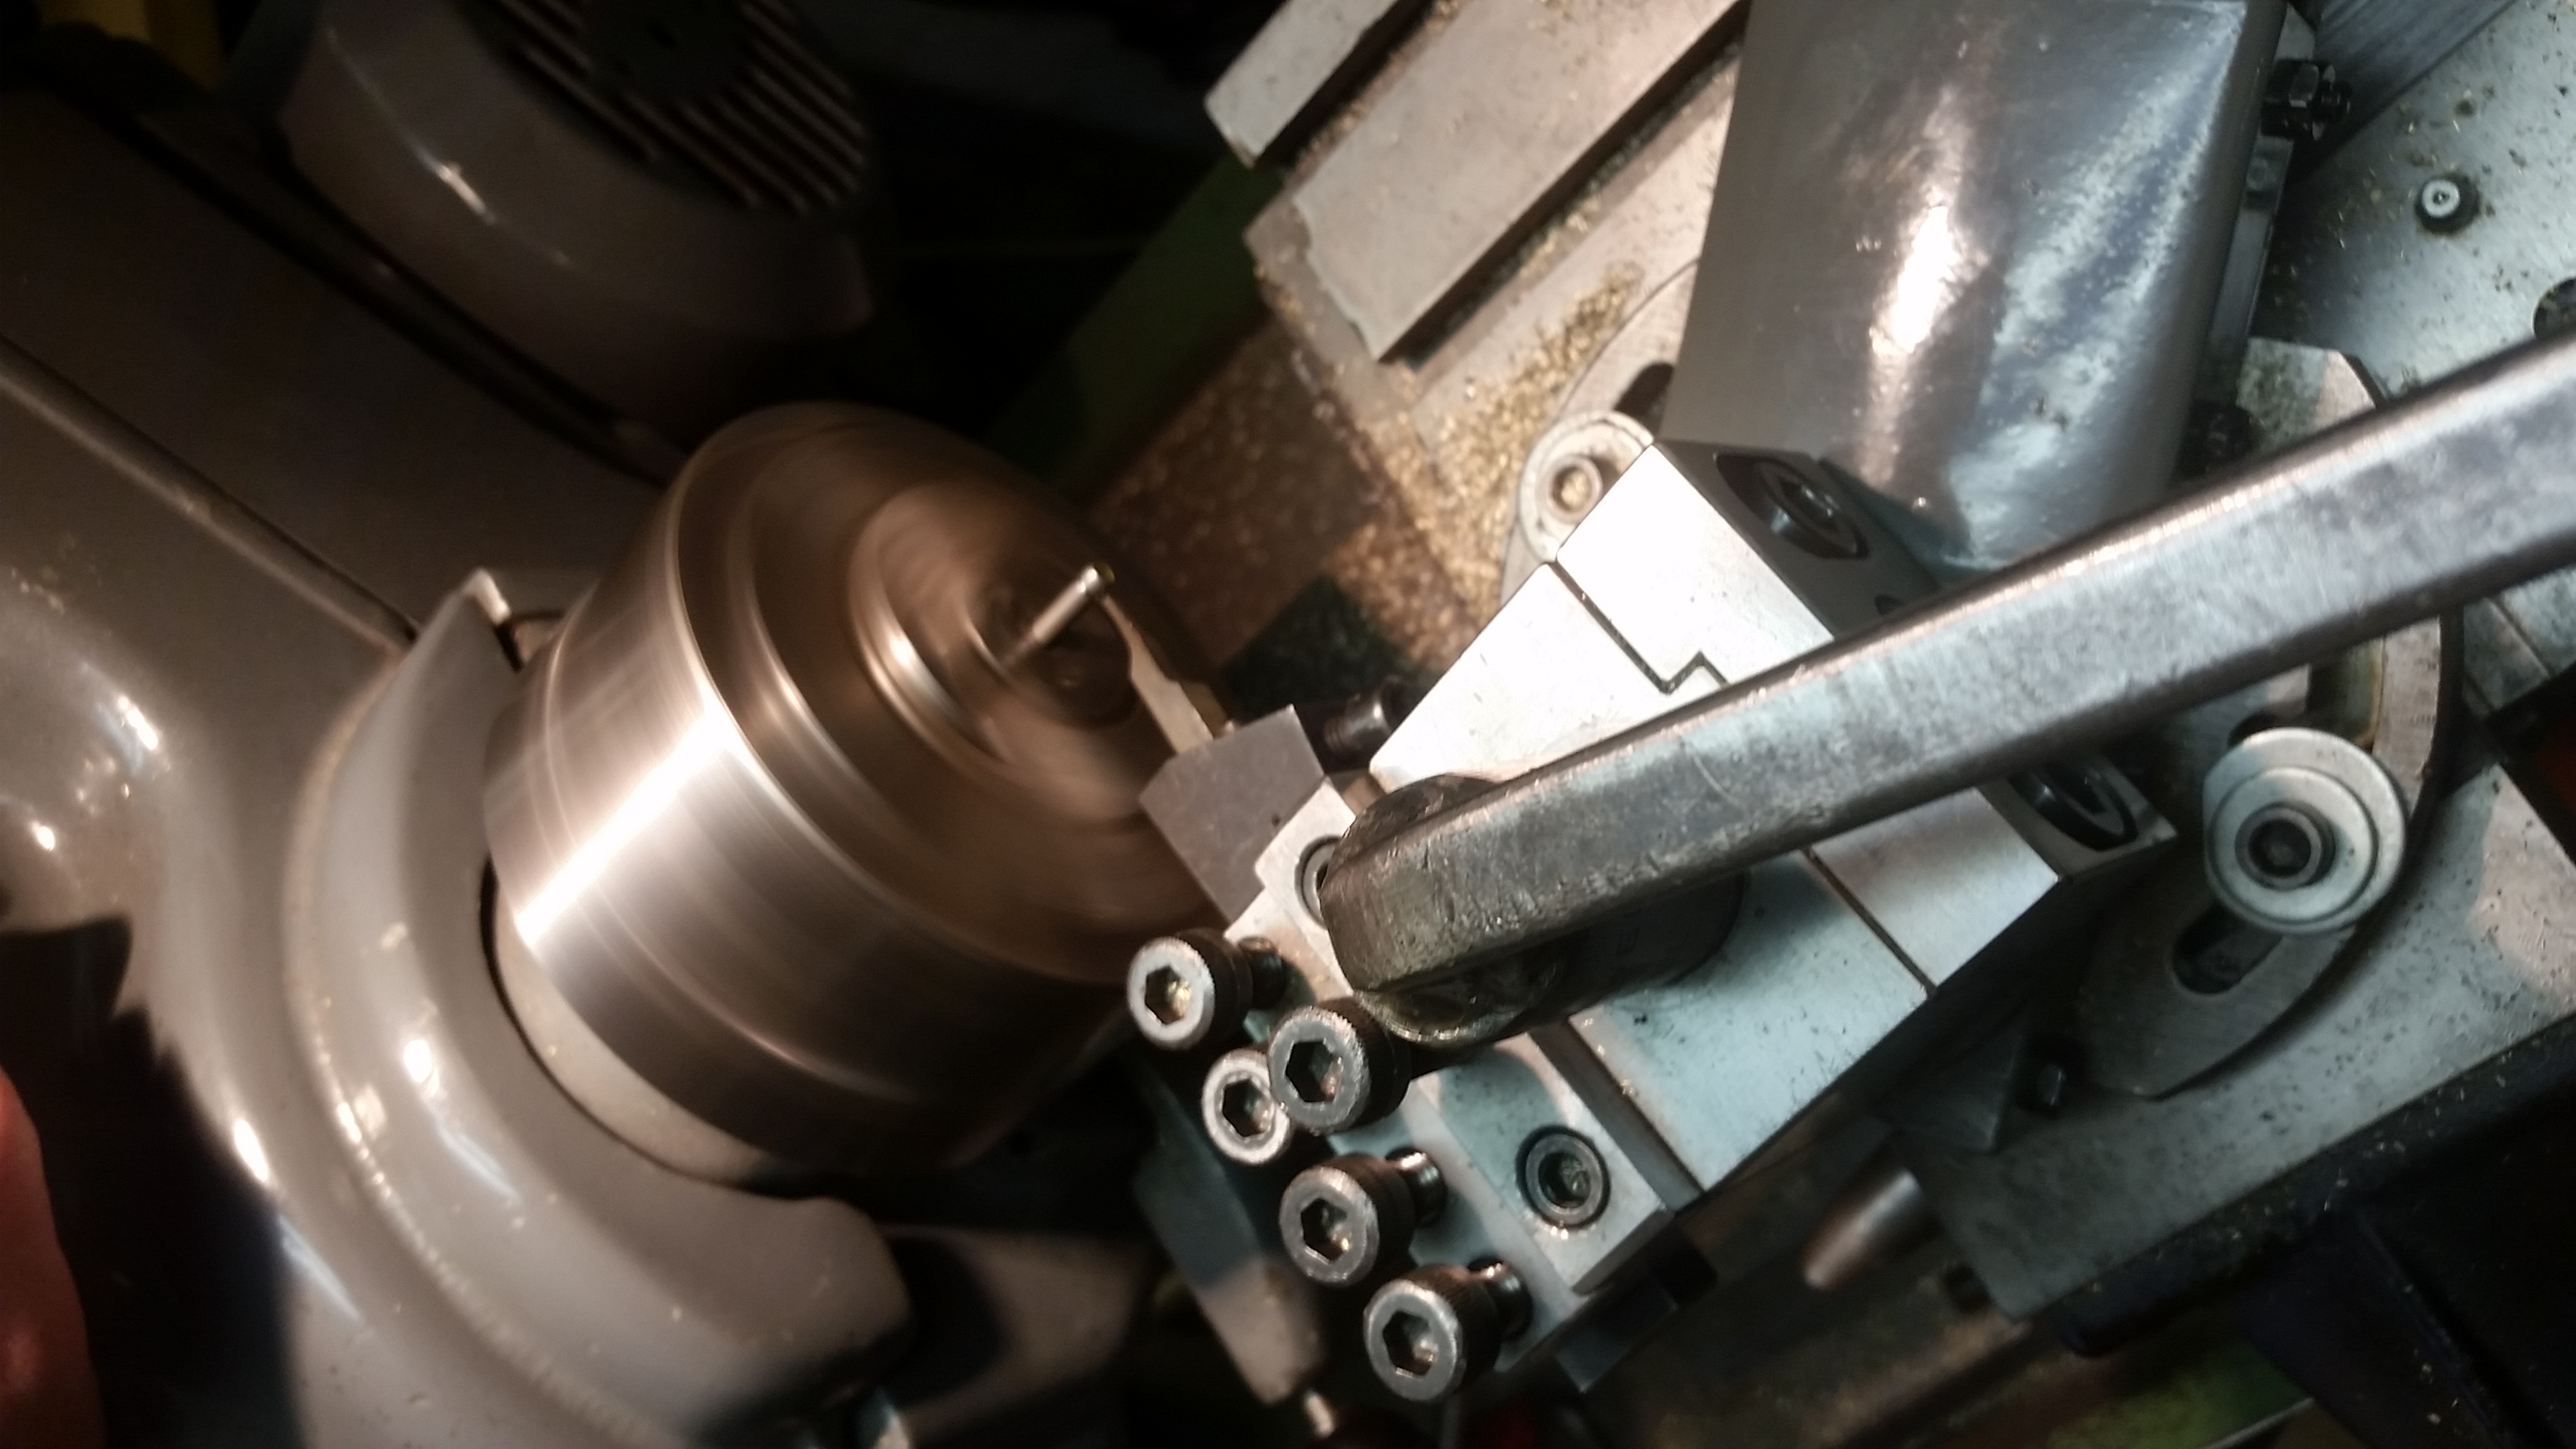
\includegraphics[width = \textwidth, angle= 270]{VAPIQ-PICTURES/latheWork}
            \caption{Lathe Work}
            %\label{fig:}
        \end{minipage}
\end{figure}
\noindent
The motor is mounted through two custom drilled holes with M3 screws and bolts. Using a lathe machine, grooves were made in the shafts to hold the C-clips which ensures that the shaft does not slide. To fit the shafts through the motor, a press machine with 20 ton capacity was used to press the shaft into position. 

\subsection{Concept 1, Conclusion}

Calculation of the thrust forces produced by the motor, mechanism, propeller combination was difficult to estimate theoretically, and therefore had to be measured empirically. The maximum thrust produced in the test rig was approximately 700g on 4 cell battery voltage, giving a max thrust of 2,4 kg. The problem was that the motor drew 18,6 A of current and quickly became overheated. The mass estimate of the quadcopter assembly was 1800g, leaving only 600g of spare thrust on maximum power and a power to weight ratio of 1,3. These factors resulted in the concept being discarded.

\subsection{Variable Pitch Concept 2}

After receiving the AXI 2208/26 motors with variable pitch mechanisms, a new concept had to be made. The new motors can produce approximately 500g of thrust each, giving a total lift of 2 kg.
\\\\
This concept consists of designing a frame that can hold all components, but as light as possible to achieve the highest power to weight ratio. The frame will be made from hybrid carbon fiber sandwich material, where the soft core material is PVC foam and the outer stiff material is carbon fiber with 12k weave and 0,90 fiber orientation.
\\\\
Legs with servo holders, as well as component brackets will be 3D-printed.

\begin{figure}[H]
        \centering
                \begin{minipage}[b]{0.4\textwidth}
            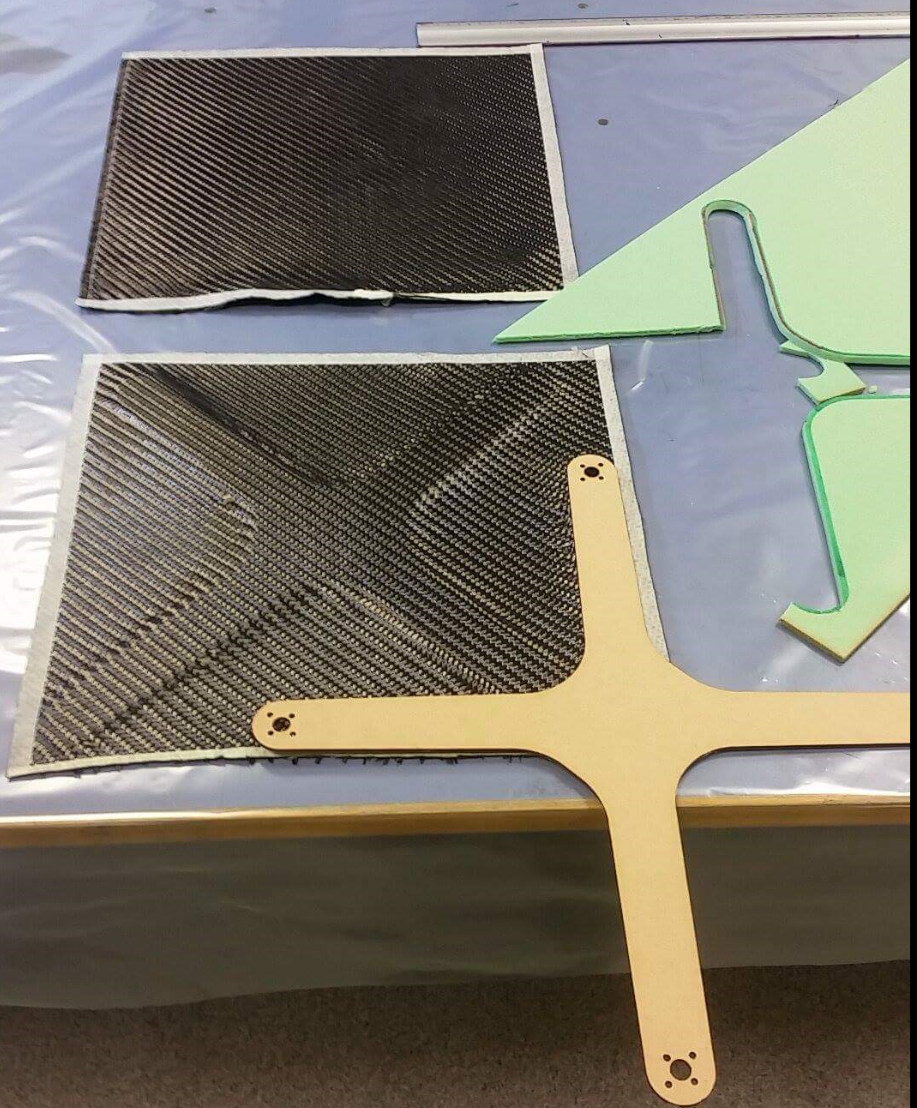
\includegraphics[width = \textwidth, angle= 0]{VAPIQ-PICTURES/MakingVPQFrame.PNG}
            \caption{Making VPQ Frame}
            %\label{fig:}
                    \end{minipage}
                 \hfill
         \begin{minipage}[b]{0,35\textwidth}
            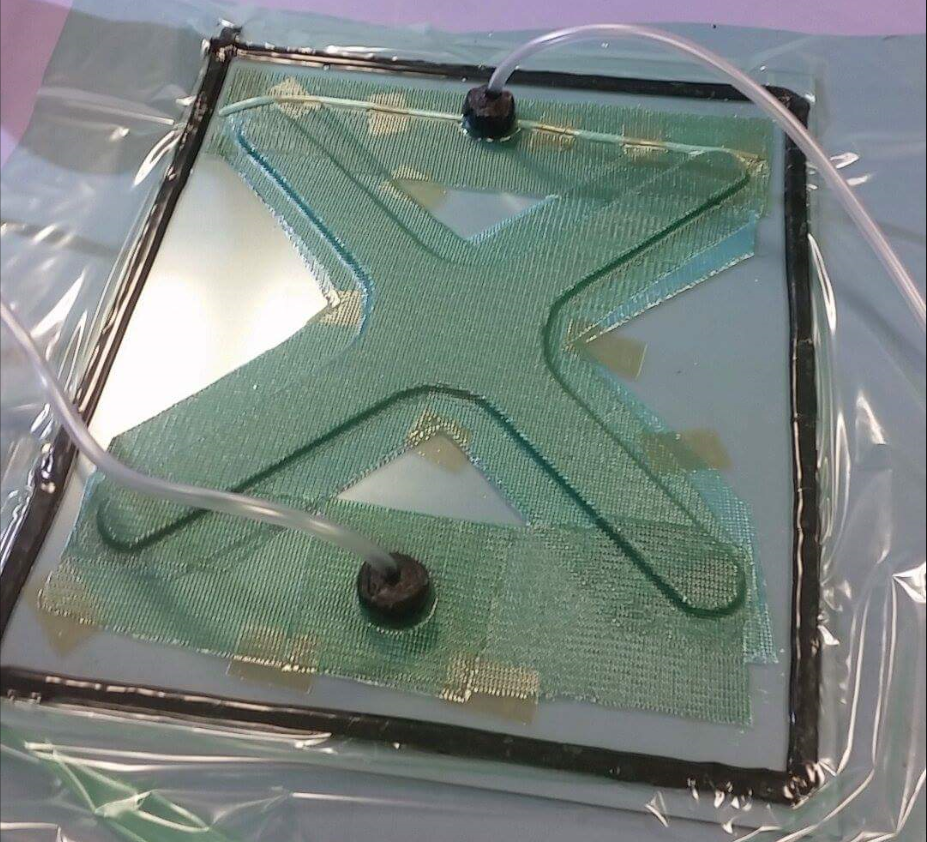
\includegraphics[width =\textwidth, angle =0]{VAPIQ-PICTURES/VacumInfusionVPQFrame.PNG}
              \caption{Vacum Infusion of VPQ frame}
            %\label{fig:nlknl}
        \end{minipage}

\end{figure} 
% abbreviation MDF- medium density fiber?
\noindent
First a laser cut model was made in MDF, then this model was used as a outline for cutting foam and the carbon fiber cloth. This build is hand traced and cut. After gluing the carbon fiber on each side of the foam, the construction was infused with epoxy resin under vacuum and left to cure for 48 hours.

%stiffens/wheigt

\newpage



